\section{Метрики качества точечного прогноза}
\label{sec:metrics}

\subsection{Немного определений}

В контексте всего вышесказанного определимся, как же количественно
посчитать, насколько наш прогноз совпадает с фактом. Мы уже выяснили,
что важны не только конкретные значения метрик, но и их стабильность
во времени. На время пока абстрагируемся от этой идеи и напомним, что
же метрики качества есть такое.

Допустим, мы построили некоторый предиктивный алгоритм. Мы можем
применить его к нашему ряду на некоторой тестовой выборке.

\begin{figure}[htb]
  \centering
  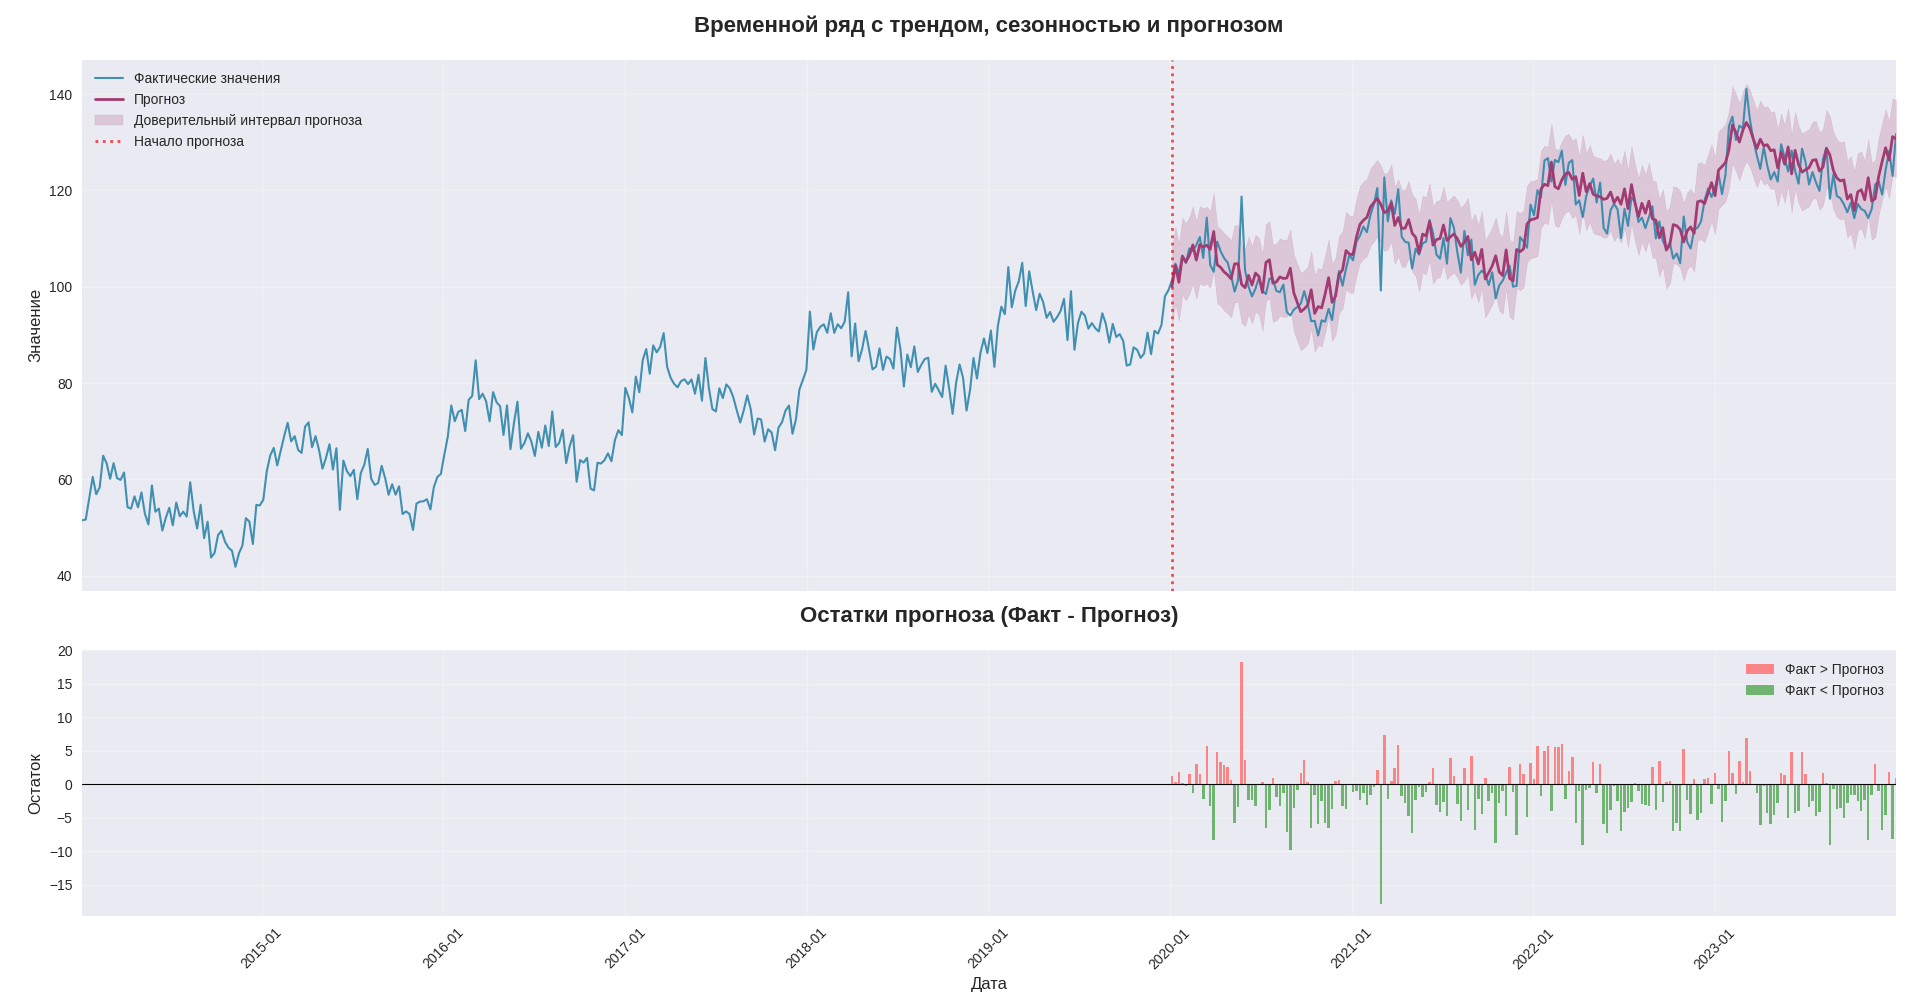
\includegraphics[width=1\textwidth]{images/forecast_errors.png}
  % \textcolor{myorange}{\textbf{\caption{Figure
  % Descriptiondas}}}\label{fig:2} % ЦВЕТ НЕ ОТРАБОТАЛ
\end{figure}

В правой нижней части графика отображены ошибки прогноза в виде барчарта.
Анализ остатков, критически важная вещь в классическом машинном
обучении / эконометрике, в случае временных рядов играет еще большую
роль, ведь в этом случае необходимо также проверять, что в ошибках
нет смещения по времени измерения. Например, в нашем случае в
остатках есть четкая сезонная составляющая - присутствие этого
паттерна говорит нам, что наша предиктивная модель была построена не
лучшим образом. Мы хотим, чтобы остатки были случайны, чтобы в них не
наблюдались никакие ярко выраженные паттерны.

Теперь перейдем к пониманию, зачем нужны метрики качества. Мы видим,
что ошибки прогноза на тестовой выборке отличаются: какие-то из них
отрицательные, какие-то положительные, какие-то имеют
высокоамлитудные, какие-то близки к нулю. Конечно, мы бы хотели,
чтобы все остатки прогноза были близки к нулю. На практике однако
подобное недостижимо, поэтому нам нужен некоторая функция агрегация,
которая бы значения всех этих остатков превратила в одно число. Тогда
мы могли бы сравнивать различные модели по тому, насколько это число
больше или меньше. Данная функция как правило задается двумя
компонентами: выбором функции потерь для индивидуального прогноза и
способа их агрегации. Выбор способа агрегации влияет на то, как
сильно мы ценим то или иное отклонение факта от прогноза. Скажем, мы
можем ценить негативное отклонение факта от прогноза сильнее, чем
позитивное - в таком случае мы будем использовать что-то вроде
квантильной функции потерь. Мы также можем ценить большие отклонения
сильнее чем небольшие - в таких случаях мы скорее всего будем
использовать что-то вроде MSE вместо MAE. От способа агрегации
функций потерь зависит то, какие наблюдения с какими отклонениями мы
ценим выше. Скажем, если в качестве способа агрегации мы выбрали
среднее, мы ценим все наблюдения в тестовой выборке одинаково. Если
же мы выберем в качестве метода агрегации, например, 95\% квантиль
распределения, то мы будем ценить больше наблюдения с
высокоамлитудными отклонениями.

Если говорить кратко, метрики качества задают то, насколько мы ценим
те или иные ошибки. Исходя из бизнес-цели, мы можем подобрать ту или
иную метрику качества. По сути различие между конкретными
функционалами качества заключается
в том, какие ошибки считаются более, а какие менее приоритетными.

Можно также сказать, что метрики качества - это дескриптивные
статистики распределения остатков.

\ex{Общеизвестный пример}{
  Про прогноз запасов товаров на складе
}

Закономерно вытекает определение выбросов модели

\defn{Выбросы (или аномалии)}{
  Выбросы - это outliers гистограммы распределения остатков
}

Когда выбросы определяются на основании гистограмм исходных данных, с
последующим применением чего-то вроде правила трех сигм, в качестве
прогнозной модели неявно предполагается константная модель.

метрики качества моделей
временных рядов как некоторые дескриптивные статистики распределения
остатков модели. аномалии сюда же (выбросы распределений).
Стьюдентизированные остатки?

\url{https://mlgu.ru/3091/}

Чекни также Бабушкина, раздел про метрики, там про ряды как раз

TODO: добавить ссылки на вшэ, гевиссту, сайт выше

TODO: написать про свойства метрик качества. типа интерпретируемости,
симметричности, устойчивости к выбросам и тд и в конце привести
сводную таблицу. Выделить классы эквивалентности

\subsection{Самые распространенные метрики качества прогноза}

Основная задача, с которой мы будем сталкиваться в данным курсе -
задача регрессии. Способов посчитать близость двух чисел
(прогноза и истинного ответа) достаточно много, и поэтому при
обсуждении регрессии у нас возникнет большое количество функционалов ошибки.
Напомним также, что в случае регрессии (в частности, в прогнозе
временных рядов) функционал и метрика качества
зачастую оказывается одним и тем же: мы можем рассматривать
среднеквадратичную ошибку как в качестве цели для оптимизации, так
и в качестве оценки итогового качества модели. При этом не все
метрики качества окажутся легко интерпретируемыми.

Чтобы обучать регрессионные модели временного ряда, нужно
определиться, как именно измеряется качество предсказаний. Будем
обозначать через \( y \) значение целевой переменной, через \( \hat{y_t} \) --
прогноз модели.
Рассмотрим несколько способов оценить отклонение \( L(y, \hat{y_t}) \)
прогноза от истинного ответа.

\subsection*{MSE и \( R^2 \)}
Основной способ измерить отклонение — посчитать квадрат разности:

\[ L = (\hat{y_t} - y)^2 \]

Благодаря своей дифференцируемости эта функция наиболее часто
используется в задачах регрессии. Основанный на ней функционал
называется среднеквадратичным отклонением (mean squared error, MSE):

\[ \text{MSE} = \frac{1}{T} \sum_{t=1}^{T} (\hat{y_t} - y_t)^2 \]

Отметим, что величина среднеквадратичного отклонения плохо
интерпретируется, поскольку не сохраняет единицы измерения — так,
если мы предсказываем цену в рублях, то MSE будет измеряться в
квадратах рублей. Чтобы избежать этого, используют корень из
среднеквадратичной ошибки (root mean squared error, RMSE):

\[
  RMSE = \sqrt{\frac{1}{T} \sum_{i=1}^{T} (\hat{y_t} - y_t)^2}.
\]

Среднеквадратичная ошибка подходит для сравнения двух моделей или для
контроля качества во время обучения, но не позволяет сделать выводы о
том, насколько хорошо данная модель решает задачу. Например, MSE = 10
является очень плохим показателем, если целевая переменная принимает
значения от 0 до 1, и очень хорошим, если целевая переменная лежит в
интервале (10000, 100000). В таких ситуациях вместо
среднеквадратичной ошибки полезно использовать коэффициент
детерминации (или коэффициент $R^2$):

\[
  R^2 = 1 - \frac{\sum_{t=1}^{T} (\hat{y_t} -
  y_t)^2}{\sum_{i=t}^{T} (y_t - \bar{y})^2},
\]

где $\bar{y} = \frac{1}{T} \sum_{t=1}^{T} y_t$ — среднее значение
целевой переменной. Коэффициент детерминации измеряет долю дисперсии,
объяснённую моделью, в общей дисперсии целевой переменной.
Фактически, данная мера качества — это нормированная
среднеквадратичная ошибка. Если она близка к единице, то модель
хорошо объясняет данные, если же она близка к нулю, то прогнозы
сопоставимы по качеству с константным предсказанием.

\subsection*{MAE}
Заменим квадрат отклонения на модуль:

\[
  L = |\hat{y_t} - y|
\]

Соответствующий функционал называется средним абсолютным отклонением
(mean absolute error, MAE):

\[
  MAE = \frac{1}{T} \sum_{t=1}^{T} |\hat{y_t} - y_t|.
\]

Модуль отклонения не является дифференцируемым, но при этом менее
чувствителен к выбросам. Квадрат отклонения, по сути, делает особый
акцент на объектах с сильной ошибкой, и метод обучения будет в первую
очередь стараться уменьшить отклонения на таких объектах. Если же эти
объекты являются выбросами (то есть значение целевой переменной на
  них либо ошибочно, либо относится к другому распределению и должно
быть проигнорировано), то такая расстановка акцентов приведёт к
плохому качеству модели. Модуль отклонения в этом смысле гораздо
более терпим к сильным ошибкам.

\subsection*{MAPE и SMAPE.}
В задачах прогнозирования нередко измеряется
относительная ошибка. Во-первых, это удобно для интерпретации — легко
понять, что «ошибка 50\%» соответствует отклонению в полтора раза от
целевой переменной. Во-вторых, это позволяет работать с разными
масштабами. Например, мы можем решать задачу прогнозирования спроса
на товары в магазине, и какие-то товары могут продаваться штуками, а
какие-то — тысячами. Чтобы при усреднении ошибок более популярные
товары не оказывали большее влияние на результат, следует
использовать функции потерь, не зависящие от масштаба. Типичный
пример относительной функции потерь:

\[
  L = \frac{|y_t - \hat{y_t}|}{y_t}
\]

Соответствующий функционал называется средней абсолютной процентной
ошибкой (mean absolute percentage error, MAPE).

У MAPE есть проблема с несимметричностью: скажем, если $y = 1$ и все
прогнозы неотрицательные, то максимальная ошибка при занижении
прогноза ($a < y$) равна единице, а ошибка при завышении прогноза ($a
> y$) никак не ограничена сверху. Это исправляется в симметричной
модификации (symmetric mean absolute percentage error, SMAPE):

\[
  L = \frac{|y - \hat{y_t}|}{(|y| + |\hat{y_t}|)/2}
\]

TODO: квантильная функция

\subsection{Для тех, кому все еще мало}

Как уже было сказано ранее, метрик качеств для временных рядов можно
придумать бесконечное количество. Ниже мы приведем менее
распространенные метрики качества прогноза, а также дадим краткое
объяснение, зачем они нужны.

TODO: написать также про следующие метрики (взято у гевиссты, их
  дохуя, поэтому надо расписать, для чего вообще они нужны + возможно
построить как выглядят график их функции):

\begin{enumerate}
  \item Метрики качества, которые зависят от масштаба данных
    (RMSE, MSE, MAE, MdAE, RMSLE, MSLE)
  \item Корень из среднеквадратичной ошибки (root mean squared error, RMSE)
  \item Cредняя абсолютная ошибка (mean absolute error, MAE)
  \item Медианная абсолютная ошибка (median absolute error, MdAE)
  \item Сравнение RMSE, MAE, MdAE
  \item Корень из среднеквадратичной логарифмической ошибки
    (root mean squared logarithmic error, RMSLE)
  \item Метрики качества на основе процентных ошибок
    (MAPE, MdAPE, sMAPE, sMdAPE, WAPE, WMAPE, RMSPE, RMdSPE)
  \item Cредняя абсолютная процентная ошибка
    (mean absolute percentage error, MAPE)
  \item Медианная абсолютная процентная ошибка
    (median absolute percentage error, MdAPE)
  \item Cимметричная средняя абсолютная процентная ошибка
    (symmetric mean absolute percentage error, SMAPE)
  \item Cимметричная медианная абсолютная процентная ошибка
    (symmetric median absolute percentage error, SMdAPE)
  \item Взвешенная абсолютная процентная ошибка
    (weighted absolute percentage error, WAPE)
  \item Средневзвешенная абсолютная процентная ошибка
    (weighted mean absolute percentage error, WMAPE)
  \item Корень из среднеквадратичной процентной ошибки
    (root mean square percentage error, RMSPE)
  \item Корень из медианной квадратичной процентной ошибки
    (root median square percentage error, RMdSPE)
  \item Сравнение MAPE, MdAPE, sMAPE, sMdAPE, WAPE, WMAPE,
    RMSPE, RMdSPE
  \item Метрики качества на основе относительных ошибок
    (MRAE, MdRAE, GMRAE)
  \item Средняя относительная абсолютная ошибка
    (mean relative absolute error, MRAE)
  \item Медианная относительная абсолютная ошибка
    (median relative absolute error, MdRAE)
  \item Средняя геометрическая относительная абсолютная ошибка
    (geometric mean relative absolute error, GMRAE)
  \item Сравнение MRAE, MdRAE, GMRAEV.4. Относительные метрики
    качества (RelMAE, RelRMSE)
  \item Относительная метрика MAE (relative MAE, RelMAE)
  \item Относительная метрика RMSE (relative RMSE, RelRMSE)
  \item Метрики качества на основе масштабированных ошибок
    (MASE)
  \item Средняя абсолютная масштабированная ошибка
    (mean absolute scaled error, MASE)

\end{enumerate}

\subsection{Сравнение метрик качества}

Сравнение метрик качества имеет смысл только если оно проводится статистически!

То есть с учетом распределений данных, их размера и числа попыток тестирования.

Критерий Диболда-Мариано